\documentclass[twocolumn]{article}
\usepackage{acro}
\usepackage[backend=biber]{biblatex}
\usepackage[inline]{enumitem}
\usepackage{amsmath}
\usepackage{cleveref}
\usepackage{pgfplots}
\usepackage{import}
\usepackage{booktabs}
\usepackage{makecell}
\usepackage{todonotes}
\usepackage{xcolor}
\usepackage{subcaption}
\usepackage{pgfplots}
\usepackage{pgfplotstable}
\usepackage{tabularx}

\usepgfplotslibrary{groupplots}
\usepgfplotslibrary{colorbrewer}

% Custom commands
\definecolor{gdvGreen}{HTML}{00B000}
\definecolor{gdvOrange}{HTML}{FFAA00}
\definecolor{gdvRed}{HTML}{E9002D}

\newcommand{\skill}{{\color{gdvGreen}{$\pmb{+}$}}}
\newcommand{\noskill}{{\color{gdvOrange}{$\pmb{-}$}}}
\newcommand{\snoskill}{{\color{gdvRed}{$\pmb{/}$}}}

% Layout
\setuptodonotes{inline}
\usepackage[font=small]{caption}

\pgfplotsset{every tick label/.append style={font=\footnotesize}}
\pgfplotsset{every axis label/.append style={font=\footnotesize}}
\pgfplotsset{every axis legend/.append style={font=\footnotesize}}

\renewcommand*{\bibfont}{\footnotesize}


% Preamble
% Declared acronyms
\DeclareAcronym{aac}{
  short=AAC,
  long=assistive and augmentative communication
}
\DeclareAcronym{bci}{
  short=BCI,
  long=brain-computer interface,
}
\DeclareAcronym{eeg}{
  short=EEG,
  long=elec\-tro\-en\-ce\-pha\-lo\-gra\-phy
}
\DeclareAcronym{ecog}{
  short=ECoG,
  long=elec\-tro\-cor\-ti\-co\-gra\-phy
}
\DeclareAcronym{erp}{
  short=ERP,
  long=event-related potential
}
\DeclareAcronym{als}{
  short=ALS,
  long=Amyotrophic Lateral Sclerosis
}
\DeclareAcronym{ms}{
  short=MS,
  long=Multiple Sclerosis
}
\DeclareAcronym{sma}{
  short=SMA,
  long=Spinal Muscular Atrophy
}
\DeclareAcronym{dmd}{
  short=DMD,
  long=Duchenne's Muscular Dystrophy
}
\DeclareAcronym{lis}{
  short=LiS,
  long=Locked-in Syndrome
}
\DeclareAcronym{vsa}{
  short=VSA,
  long=visuospatial attention
}
\DeclareAcronym{itr}{
  short=ITR,
  long=information transfer rate
}
\DeclareAcronym{ssvep}{
  short=SSVEP,
  long=steady-state visually evoked potential
}
\DeclareAcronym{cvep}{
  short=cVEP,
  long=code-modulated visually evoked potential
}
\DeclareAcronym{mvep}{
  short=mVEP,
  long=motion-onset visually evoked potential
}
\DeclareAcronym{vep}{
  short=VEP,
  long=visually evoked potential
}
\DeclareAcronym{csp}{
  short=CSP,
  long=common spatial patterns
}
\DeclareAcronym{cca}{
  short=CCA,
  long=canonical correlation analysis
}
\DeclareAcronym{lda}{
  short=LDA,
  long=linear discriminant analysis
}
\DeclareAcronym{rocauc}{
  short=ROC-AUC,
  long=area under the receiver-operator characteristic curve
}
\DeclareAcronym{snr}{
  short=SNR,
  long=signal-to-noise ratio
}
\DeclareAcronym{ica}{
  short=ICA,
  long=independent component analysis
}
\DeclareAcronym{pca}{
  short=PCA,
  long=principal component analysis
}
\DeclareAcronym{cble}{
  short=CBLE,
  long=Classifier-based Latency Estimation
}
\DeclareAcronym{wcble}{
  short=WCBLE,
  long=Classifier-based Latency Estimation with Woo\-dy iterations
}
\DeclareAcronym{tlda}{
  short=tLDA,
  long=block-Toeplitz linear discriminant analysis
}
\DeclareAcronym{lcmv}{
  short=LCMV,
  long=linearily constrained minimum-variance
}
\DeclareAcronym{isi}{
  short=ISI,
  long=inter-stimulus interval
}
\DeclareAcronym{tbi}{
  short=TBI,
  long=traumatic brain injury
}
\DeclareAcronym{fa}{
  short=FRDA,
  long=Friedreich's Ataxia
}
\DeclareAcronym{sspi}{
  short=SSPI,
  long=severe speech and physical impairment
}
\DeclareAcronym{sspgi}{
  short=SSPGI,
  long={severe speech, physical and gaze impairment}
}
\DeclareAcronym{eog}{
  short=EOG,
  long=electrooculogram
}
\DeclareAcronym{rsvp}{
  short=RSVP,
  long=rapid serial visual presentation
}
\DeclareAcronym{hoda}{
  short=HODA,
  long=Higher Order Discriminant Analysis
}
\DeclareAcronym{bttda}{
  short=BTTDA,
  long=Block-Term Tensor Discriminant Analysis
}
\DeclareAcronym{cp}{
  short=CP,
  long=cerebral palsy
}
\DeclareAcronym{mi}{
  short=MI,
  long=motor imagery
}
\DeclareAcronym{stbf}{
  short=STBF,
  long=spatiotemporal beamformer
}
\DeclareAcronym{stbf-struct}{
  short=STBF-struct,
  long=structured spatiotemporal beamformer
}
\DeclareAcronym{stbf-emp}{
  short=STBF-emp,
  long=STBF with empirical covariance
  estimation
}
\DeclareAcronym{stbf-shrunk}{
  short=STBF-shrunk,
  long=STBF with shrunk covariance estimation
}
\DeclareAcronym{loocv}{
	short=LOOCV,
	long=leave-one-out cross-validation
}
\DeclareAcronym{svm}{
	short=SVM,
	long=support vector machine
}
\DeclareAcronym{hosvd}{
	short=HOSVD,
	long=Higher Order Singular Value Decomposition
}
\DeclareAcronym{ucd}{
	short=UCD,
	long=user-centered design,
}

\addbibresource{references.bib}

\author{
	Arne Van Den Kerchove,
	Juliette Meunier,
	Marie de Moura, \\
	Alixe Willemssens,
	Hakim Si-Mohammed,
	Etienne Allart, \\
	François Cabestaing
	Marc M. Van Hulle
}

\title{Case studies on visual ERP-based brain-computer interface use by
	individuals with severe speech, physical, speech and eye movement impairments}

\begin{document}

\maketitle

\begin{abstract}
	Individuals with severe speech and physical impairment face significant challenges in
	communication and	daily interaction.
	Visual \acp{bci} offer a potential assistive solution, but their usability is
	limited when facing eye motor impairments that affect gaze fixation
	and \ac{vsa}.
	This study investigates the feasibility of a gaze-independent visual oddball
	\ac{bci} for individuals with \ac{sspgi}.
	Seven participants with varying degrees of eye motor impairments were
	recruited and \ac{bci} decoding performance evaluated under three conditions:
	overt, covert, and free \ac{vsa} using multiple classification methods.
	Results confirm that covert \ac{vsa} with central fixation leads to decreased
	performance, whereas uncued \ac{vsa} is comparable to overt \ac{vsa} in some
	gaze-impaired participants.
	Furthermore, cross-condition decoder training and evaluation suggests that training
	with overt \ac{vsa} may improve performance in gaze-impaired individuals.
	These findings highlight the need for adaptive decoding strategies and further
	validation in applied settings used by impaired individuals.
\end{abstract}

\acresetall
\section{Introduction}
Neurological conditions, such as acquired brain lesions,
neuromuscular disorders and \ac{als} can result in severe speech and physical impairment.
This, in turn, significantly alters an individual's ability to communicate and interact
with their environment, reducing the level of activity and participation,
and overall quality of life.
\Ac{aac} technology leveraging visual \acp{bci},
which relies on the interpretation of visual stimuli by the user,
offers several advantages in this context.
Visual \acp{bci} operate with non-invasive recording technology and utilize rapid stimulation.
This makes them well-suited for real-time communication tasks.
\todo{
	I am missing a few references in this paragraph. Some (older) suggestions:

	R.E.O.S. Ascari et al., “Mobile interaction for augmentative and alternative communication: A
	systematic mapping,” J Interact Syst, vol. 9, 2018.
	Schultz, T., et al. (2017). Biosignal-based spoken communication: A survey. IEEE/ACM Trans Audio, Speech, Language Process, 25(12), 2257–2271.
}

However, severe visual impairments such as nystagmus (uncontrolled eye movements), diplopia (double
vision), ophthalmoplegia (eye paralysis) fatigability and head motion
limitations can significantly hinder the ability to use visual BCIs.
These impairments make it difficult for
\ac{bci} users to track or focus on visual stimuli accurately, reducing their
performance with BCIs that rely on visual cues~\cite{McCane2014,FriedOken2020,Pasqualotto2015}.
Unfortunately, it is again for this group that eye tracking solutions also
perform poorly, making them more reliant on potential developments in \acp{bci}
that do not rely on eye gaze.\todo{reference}

Eye motor impairments are presumed to reduce performance in operating visual
\acp{bci}~\cite{VanDenKerchove2024a}, since users
cannot comfortably redirect their gaze at the desired target,
i.e., perform overt \ac{vsa}.
This is usually circumvented by designing gaze-independent~
\acp{bci}~\cite{Riccio2012}.
These interfaces either avoid visual stimulation or exploit some form of
covert \ac{vsa}, where gaze and \ac{vsa} do not coincide.

Several studies on visual oddball \acp{bci} indicate that performance declines without fixation on the intended target~\cite{Brunner2010, Treder2010, RonAngevin2019}, necessitating gaze-independent solutions.
These studies build on the assumption that \ac{bci} users with eye motor
impairment would feel comfortable operating an interface in pure covert \ac{vsa} with
central fixation.
One could argue that a \ac{bci} verified to work only with central fixation could
also be considered gaze-dependent.
This does not account for the residual eye motor capabilities of most individuals
with \ac{sspgi}, the (dis)comfort they experience while
performing gaze fixation and other confounding factors resulting from their eye
motility.

It is notable that studies reporting on
gaze-independent visual \ac{bci} use by individuals with \ac{sspgi} are very few.
Results are usually different from those obtained with healthy control
participants, due to difference in capabilities, brain
response, equipment and environment.

\textcite{Lesenfants2014} tested a \ac{bci} using gaze-independent \acp{ssvep} in six
participants with \ac{lis} yet they only exceeded chance level accuracy in two.
More recently, \textcite{Peters2020} performed a trial with two
participants with late-stage \ac{als} with severe visual impairment.
Their \ac{ssvep} paradigm was not optimized for gaze-independence, but the
system showed high accuracy, outperforming an eye tracking alternative.
It would be of interest to determine whether such results can be replicated with
participants with other neurological conditions, and with a visual oddball rather
than an \ac{ssvep} paradigm.

\textcite{Orhan2012} and \textcite{Oken2014} tested the \ac{rsvp} speller with
individuals with \ac{lis}.\todo{with what result?}

\textcite{Severens2014} evaluated the visual Hex-o-Spell~\cite{Treder2010} on 5
participants with \ac{als} and showed that this visual oddball interface optimized
for gaze-independence can outperform a tactile \ac{bci}.
While this speaks to the power of visual paradigms even in groups that are
expected to have eye motor impairment, they did not verify the gaze direction
of participants during the experiment.
It was assumed that participants were performing overtly.
Participants with \ac{als} also exhibited a substantially lower accuracy than healthy
controls (58\% vs. 88\%).

\textcite{VanDenKerchove2024} also built towards a gaze-independent solution
using the visual Hex-o-Spell interface~\cite{VanDenKerchove2024}.
They partially accounted for the fact that \ac{bci} users with \ac{sspgi} might
not fully rely on central gaze fixation by evaluating settings independent of
central fixation.
They showed gaze-independent performance can be improved in healthy subjects by
using a suited decoding strategy that corrects for latency jitter in covert \ac{vsa} responses.
Yet, there is a need for verification of these results in individuals with
\ac{sspgi}.

Ultimately, this research aims to develop gaze-independent \ac{bci} for
individuals who are fully locked-in and have no alternative means of communication.
However, this group is very small and it is often challenging to recruit them
into a study and perform experiments~\cite{Wolpaw2006}.
Individuals with less severe paralysis or in less progressed disease stages that struggle with
eye-tracking technology could also benefit from
solutions tailored to their specific situation and remaining capabilities.
Therefore, we apply the concepts from earlier work and literature to
individuals with severe speech and physical impairment affected by various degrees of eye motor impairment
using a visual oddball \ac{bci}.
The objectives of this study are as follows:
\begin{enumerate*}[label={(\arabic*)}]
	\item Explore the capabilities and experienced comfort of individuals with
	      \ac{sspgi} when operating a visual \ac{bci},
	\item evaluate the performance of a gaze-independent visual \ac{bci} for this
	      group,
	\item verify if this performance can be improved with a suitable decoding
	      strategy.
\end{enumerate*}

\begin{table}
	\footnotesize
	\printacronyms[template=tabular, heading=none]
	\caption{List of acronyms.}
\end{table}


\section{Materials \& methods}
\subsection{Recruitment}
Participants were recruited from the Neuromuscular Reference center at
University Hospital Leuven (Leuven, Belgium), TRAINM Neuro Rehab Clinics
(Antwerp, Belgium), the Neurorehabilitation Unit at the Lille University
Medical Center (Lille, France), and Fondation Partage et Vie (Loos,
France).
Ethical approval for this multi-center study was obtained from the Ethics
Commission of the University Hospital Leuven (S62547).
Experiments were performed under the supervision of the treating physician.

In order to be recruited, participants must:
\begin{enumerate}
	\item be at least 18 years old and no older than 60
	      years,
	\item belong to class 2 or 3 according to the \ac{bci}	user selection criteria
	      presented by~\textcite{Wolpaw2006},
	      \label{item:patients/inclusion/wolpaw}
	\item have limitations to the extent or comfort of their eye motor control
	      (partial or full gaze paralysis, uncontrolled gaze movements, or conditions affecting the capability to direct the gaze or fixate.)
	      \label{item:patients/inclusion/oculomotor}
	\item have given their informed consent prior to participation.
\end{enumerate}
Participants were excluded if they:
\begin{enumerate}
	\item had a diagnosis of a major medical condition, including any major
	      neurological or psychiatric disorder other than those of interest based on
	      inclusion criteria~\ref{item:patients/inclusion/wolpaw},
	      and~\ref{item:patients/inclusion/oculomotor}\label{item:patients/exclusion/medical}
	\item had a predisposition to or a history of any kind of epileptic seizures,
	      including photosensitive epilepsy,\label{item:patients/exclusion/epilepsy}
	\item had a severe loss in vision or hearing that would significantly impair
	      participation in the experiment,\label{item:patients/exclusion/vision}
	\item were using specific psychoactive medications or substances that could affect the outcome.
	      (neuroleptics or benzodiazepines)
	      \label{item:patients/exclusion/cognitive}
	\item were unable to understand the experiment instructions and cooperate,
	\item had any other limitations preventing them from performing the given task.
\end{enumerate}

In total, 11 individuals were contacted. Of these, one person with
\ac{ms} was excluded based on criterion~\ref{item:patients/exclusion/vision}.
One person recovering from \ac{tbi} was excluded based on both~\ref{item:patients/exclusion/epilepsy}
and~\ref{item:patients/exclusion/cognitive}, and one person recovering from
stroke based on~\ref{item:patients/exclusion/medical}.
One further person recovering from a stroke was excluded due to technical
difficulties during the experimental session.

Ultimately, 7 participants were retained.
Of these, one participant was diagnosed with bulbar-onset \ac{als}, three with
\ac{fa} an three were recovering from \ac{lis} due to stroke.
Table~\ref{tab:patients/patients} lists the included participants and their
diagnoses.
\begin{table*}[t]
	\centering
	\footnotesize
	\footnotesize
\begin{tabularx}{\linewidth}{@{}Xlrrrlllrr@{}}
	\toprule
	\textbf{ID}     & \textbf{Diagnosis}            & \textbf{Age}           & \textbf{Sex} & \textbf{Hand.} &
	\textbf{Speech} & \textbf{Trach.}               & \textbf{Communication} &
	\textbf{W}      & \textbf{KB}                                                                                                                      \\ \midrule
	PA1             & bulbar-onset \acs{als}        & 58                     & M            & L              & anarthric  & no  & tablet       & 3 & 4 \\
	PB1             & \acs{fa}                      & 41                     & M            & L              & dysarthric & no  & verbal       & 3 & 3 \\
	PB2             & \acs{fa}                      & 43                     & F            & R              & dysarthric & no  & verbal       & 3 & 3 \\
	PB4             & \acs{fa}                      & 48                     & M            & R              & dysarthric & no  & verbal       & 3 & 3 \\
	PC2             & ischemic brainstem stroke     & 43                     & M            & R              & anarthric  & yes & eye movement & 2 & 4 \\
	PC3             & haemorrhagic brainstem stroke & 43                     & F            & R              & anarthric  & yes & letterboard  & 2 & 3 \\
	PC4             & ischemic brainstem stroke     & 54                     & M            & R              & anarthric  & yes & letterboard  & 2 & 3 \\
	\bottomrule
\end{tabularx}

	\caption{Included participants with their diagnosis and relevant communication
		capabilities.
		Trach.: underwent a tracheostomy, W: classification according
		to~\textcite{Wolpaw2006}, KB: classification according
		to~\textcite{Kuebler2008}.
	}
	\label{tab:patients/patients}
\end{table*}

\subsection{Visual skills and eye motor examination}

Self-reported eye motor and visual abnormalities as reported in~\cref{tab:patients/eye}
were recorded according to the relevant visual \ac{bci} skills presented by~\textcite{FriedOken2020}.
\todo{Clearly define visual skill with reference to paper}
\todo{Visual skills is maybe a broad terms as it also refers to cortical issues.}
These include visual acuity, visual fixation, eyelid function, ocular motility,
binocular vision, and field of vision.
Additionally, participants and their caregivers were asked about eye tremors
(nystagmus or other) and other involuntary eye movements.
Vision was assessed using a logMAR chart~\cite{Bailey1976}.
%As an objective metric, we implemented and performed the automated NeuroEye eye movement
%test proposed by~\textcite{Hassan2022} using calibration-free eye tracking to
%check if it revealed any further eye motor abnormalities.
%This was not the case.
\begin{table*}[t]
	\begin{tabular}{@{}lccccccc@{}}
	\toprule
	                     & PA1      & PB1      & PB2       & PB4      & PC2       & PC3       & PC4       \\
	\midrule
	Visual fixation      & \noskill & \noskill & \noskill  & \noskill & \noskill  & \noskill  & \noskill  \\
	Eyelid function      & \skill   & \skill   & \skill    & \skill   & \skill    & \noskill  & \noskill  \\
	Ocular motility      & \skill   & \noskill & \skill    & \noskill & \snoskill & \snoskill & \noskill  \\
	Binocular vision     & \skill   & \skill   & \skill    & \skill   & \noskill  & \snoskill & \snoskill \\
	Field of vision      & \skill   & \skill   & \skill    & \skill   & \skill    & \snoskill & \noskill  \\
	Involuntary movement & \skill   & \noskill & \snoskill & \noskill & \noskill  & \noskill  & \skill    \\
	\midrule
	Visual acuity        & 0.0      & 0.0      & 0.6       & 0.2      & 0.0       & 0.0       & 0.6       \\
	\bottomrule
\end{tabular}

	\caption[Visual skills of the included participants.]{%
		Self-reported visual skills as defined by \textcite{FriedOken2020} of
		gaze-impaired participants included in this study.
		\skill\ skilled, \noskill\ impaired, \snoskill\ severely impaired.
		Visual acuity was assessed using the logMAR scale (lower is better).}
	\label{tab:patients/eye}
\end{table*}

All participants reported some degree of fatigue or discomfort when fixating.
Participant PA1 had the mildest impairment, only reporting fatigue when fixating
for prolonged times.
The \ac{fa} participants were mostly affected by eye tremors and impaired pursuit.
PB2 suffered from especially severe horizontal oscillating involuntary eye
movements.
Eye motor function of participants PC2, PC3, and PC4 was most severely affected.
Participant PC2 was only able to look up and down and had a deviation in the
left eye causing diplopia, but this was corrected by a prism glass.
Participant PC3 only retained partial motility of the right eye, while the left eye was permanently closed.
Participant PC4 had one deviated eye with a corneal abscess affecting the motility
and vision in the right eye, and reducing motility in the left.

Finally, we also recorded gaze position throughout the experimental session to
register the participant's gaze relative to the stimulated \ac{bci} targets,
using a Tobii X2-30 Compact (Tobii
Technology AB, Sweden) portable eye tracker placed at the bottom of the laptop screen.
The registered data was cleaned by fusing left and right eye screen-based gaze
coordinates into one channel for the horizontal and one for vertical gaze position.
If both were present for a given sample, the fused channel was the mean of both
values.
If at a given sample either the left or the right eye was not detected for a
given channel, the value of the other one was adopted.
If both were missing, the gaze position remained unset at that time point, and no
interpolation was performed.



\subsection{\Acs{bci} stimulation}

The \ac{bci} stimulation procedure was based on the
Hex-o-Spell~\cite{Treder2010} implementation presented
by~\textcite{VanDenKerchove2024}.
Similar to this study, the task consists of counting the flashes of a cued
target among 6 circular, flashing targets laid out in a hexagonal pattern in the
field of view of the user as displayed
in~\cref{fig:methods/stimulation/stimulation}.
We refer to \textcite{VanDenKerchove2024} for further details on the implementation
of the stimulation procedure.
\begin{figure*}[t]
	\centering
	\begin{subfigure}[b]{.41\textwidth}
		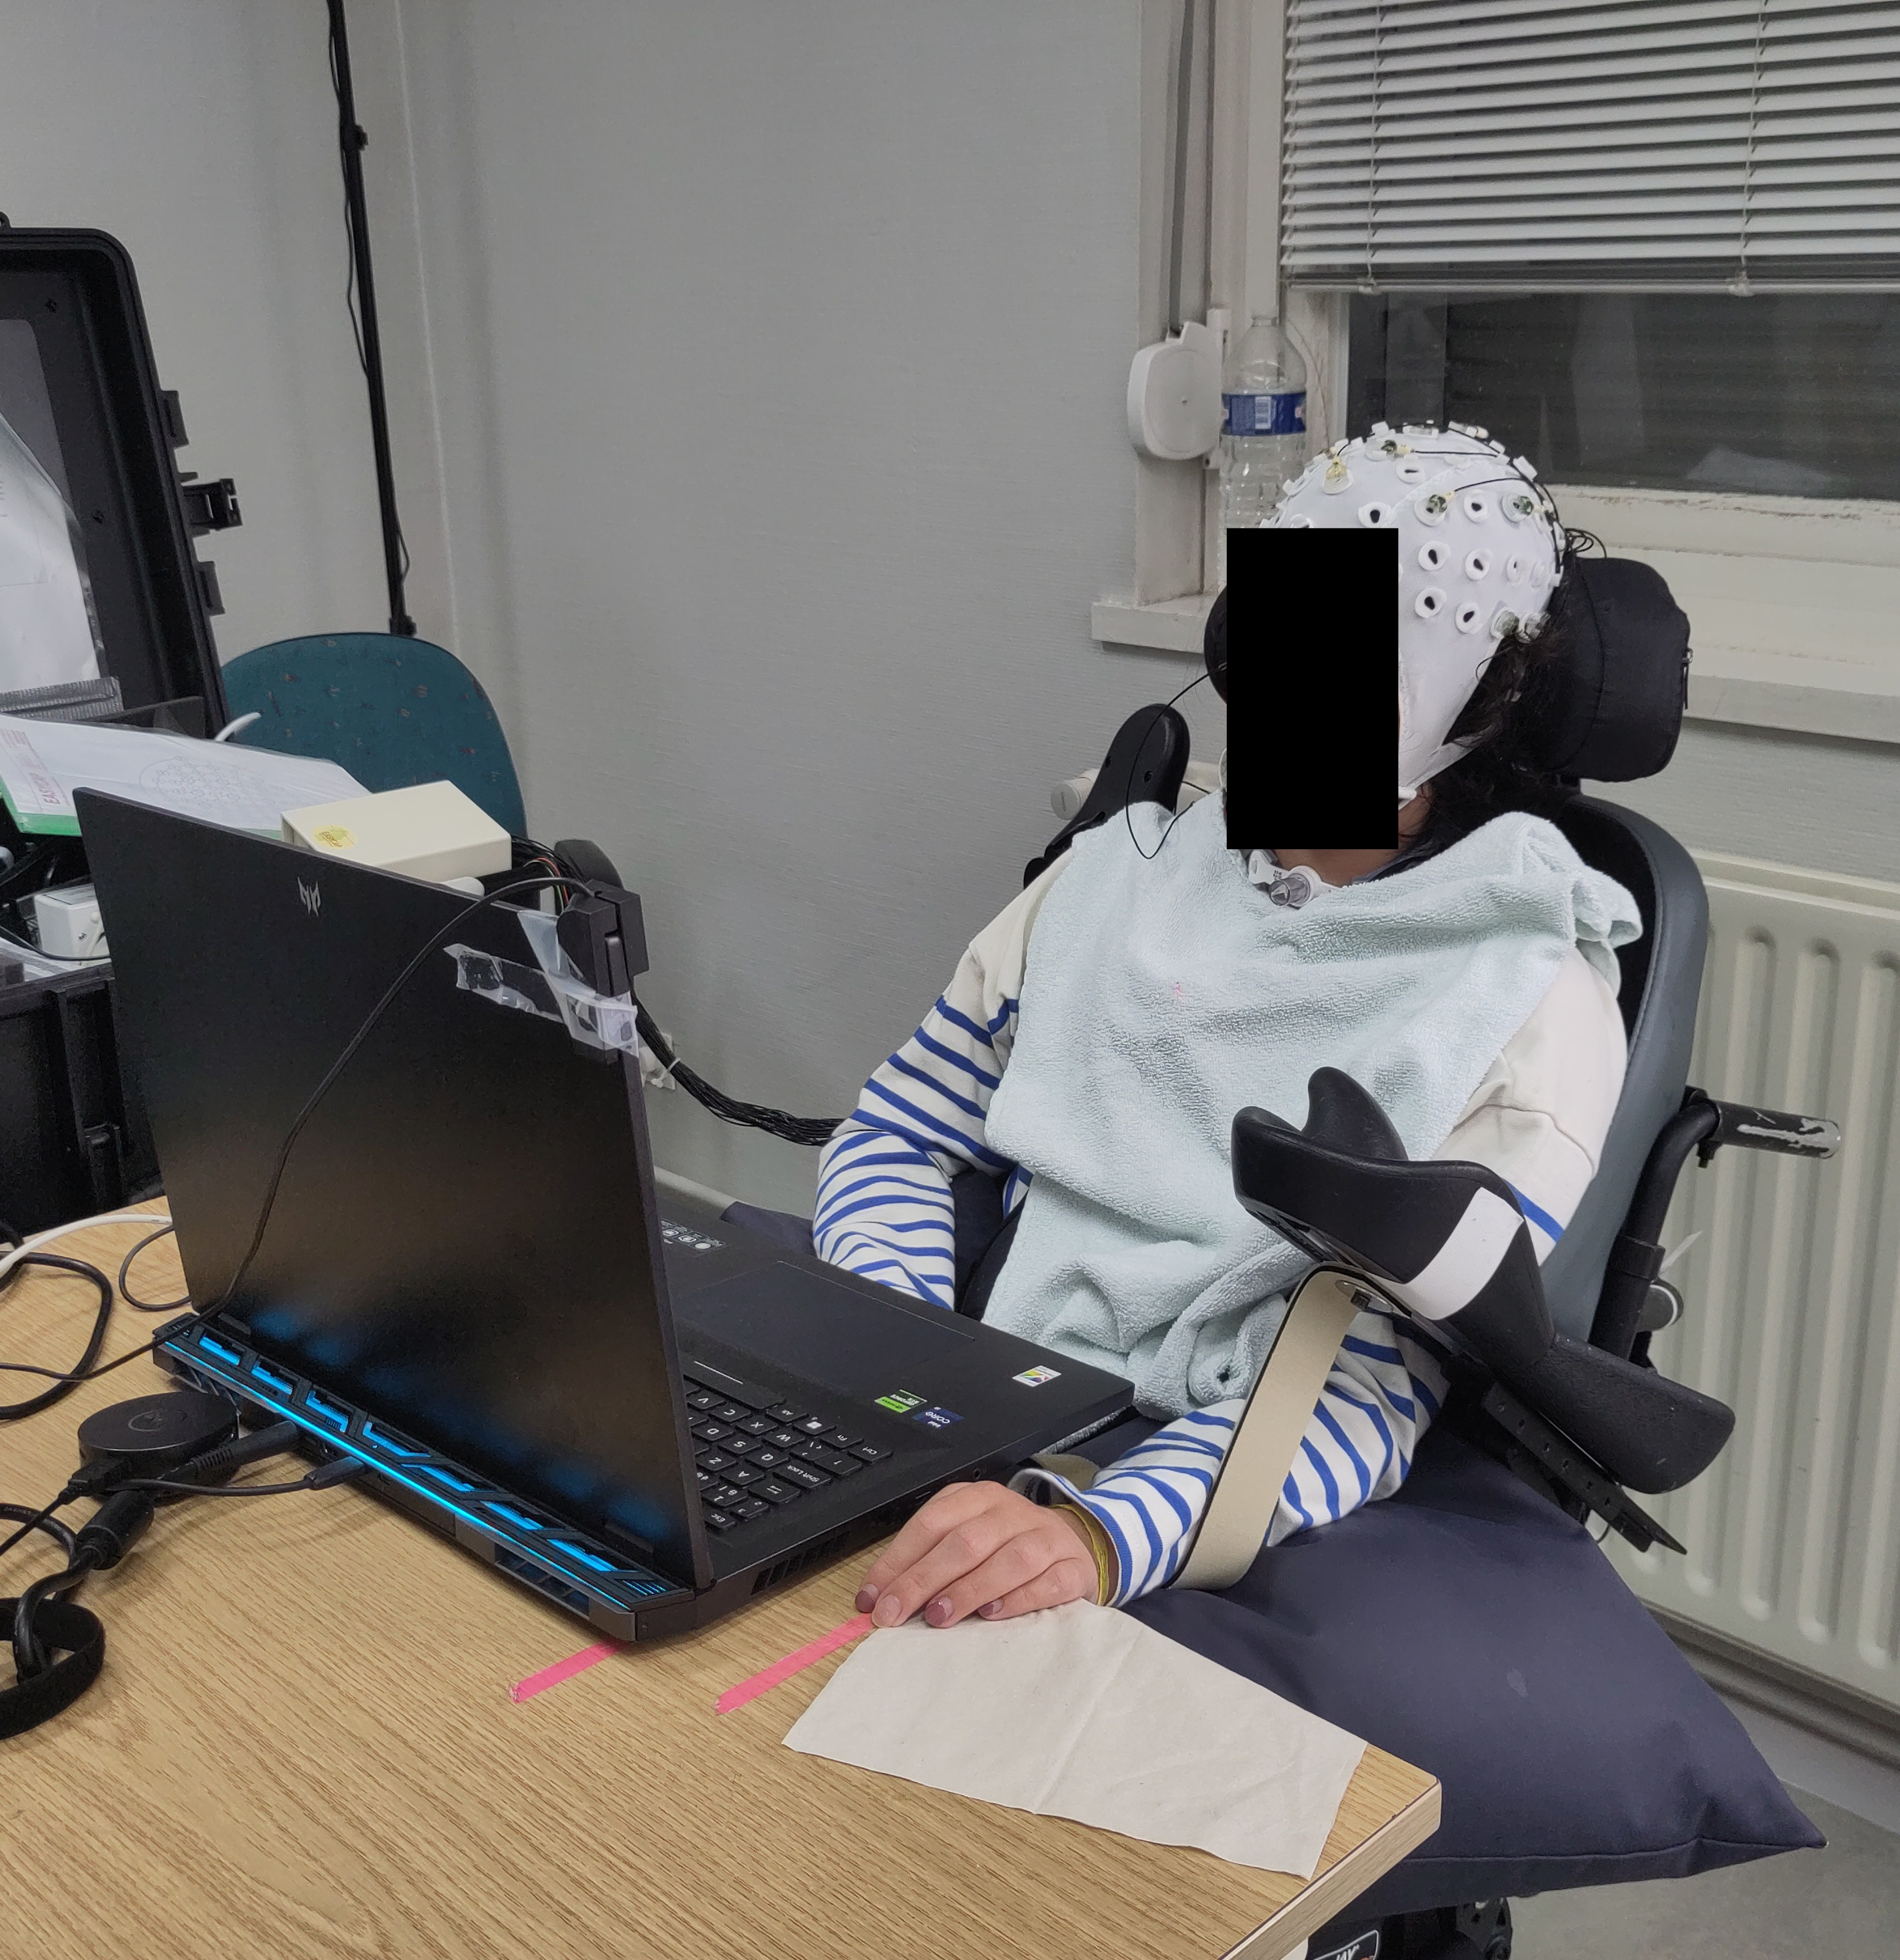
\includegraphics[width=\textwidth]{figures/PD01b-obfuscated.jpg}
		\caption{A participant seated in a wheelchair in front of the stimulation laptop with EEG
			cap.}
	\end{subfigure}\hfill%
	\begin{minipage}[b]{.54\textwidth}
		\begin{subfigure}[b]{.45\linewidth}
			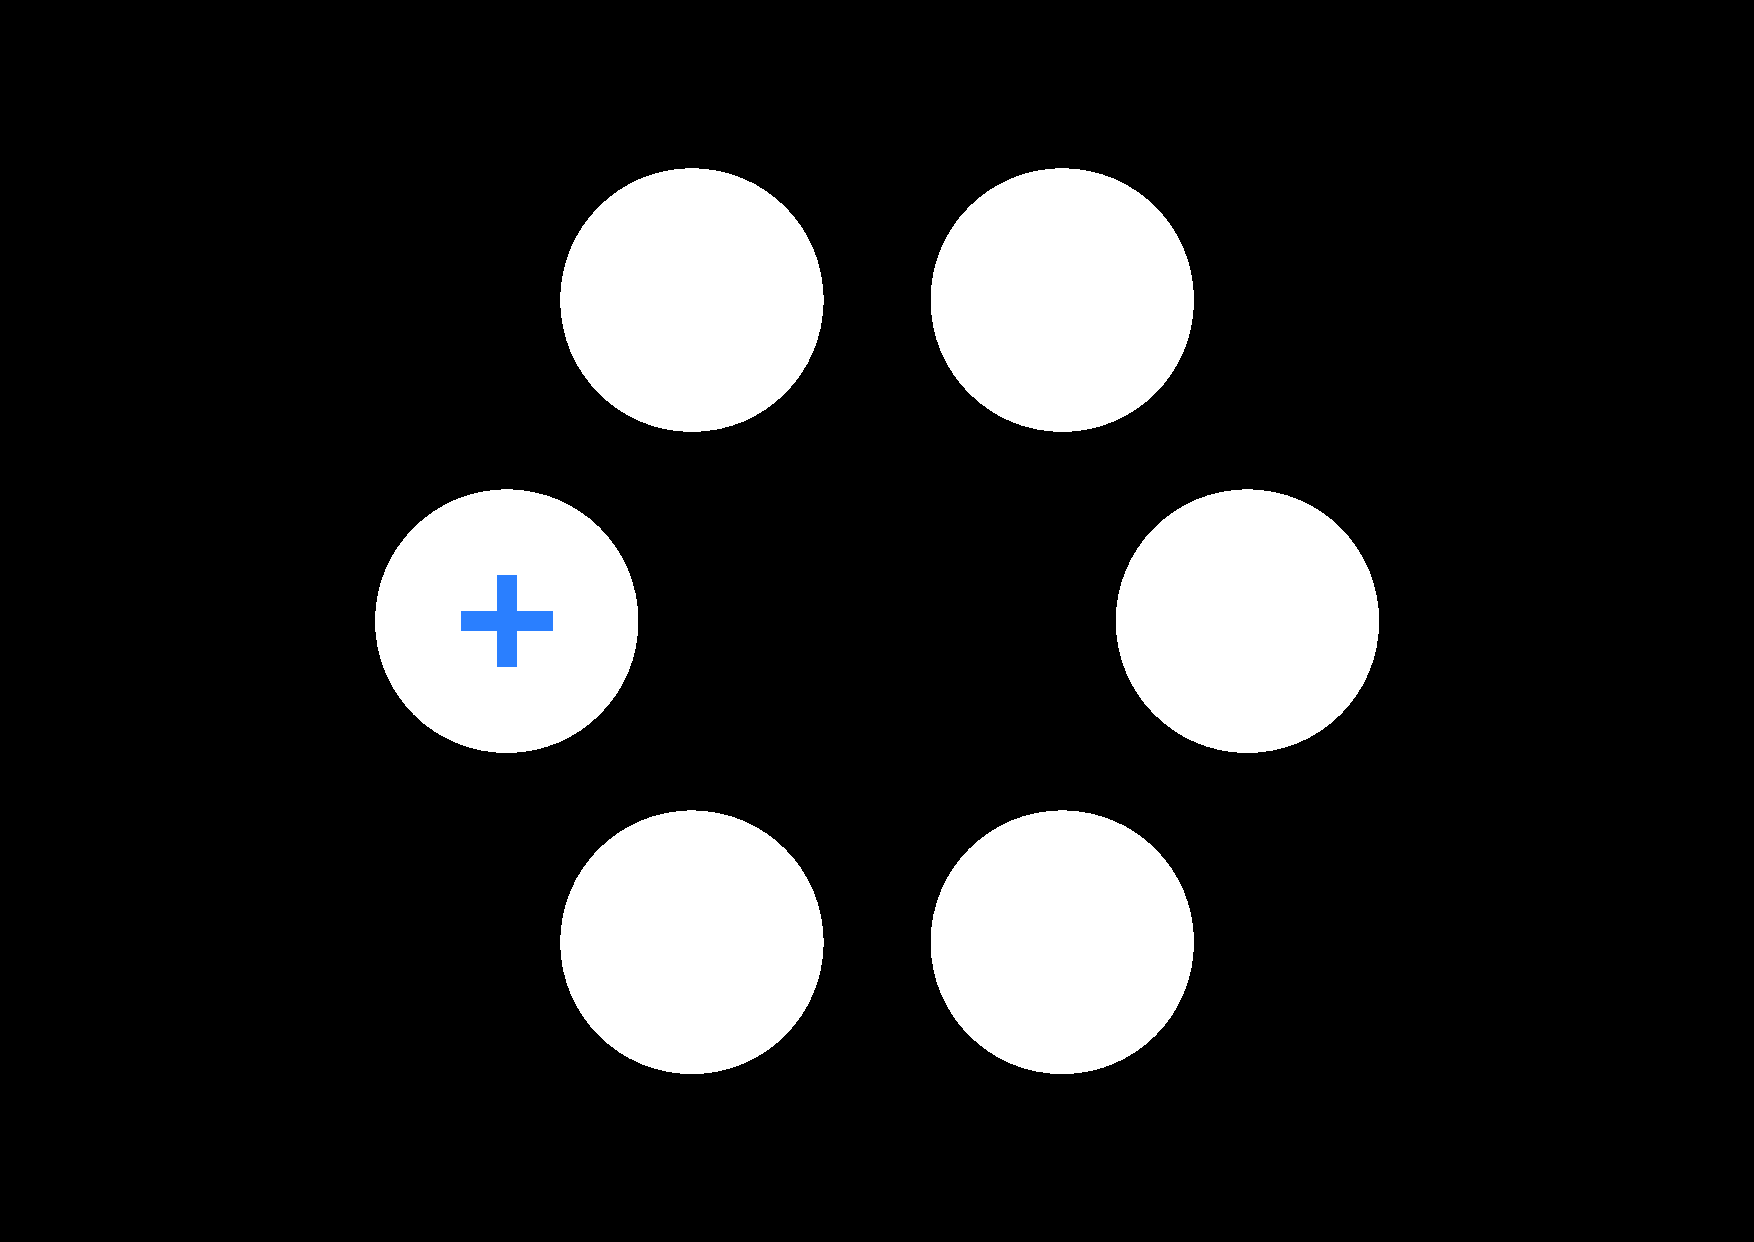
\includegraphics[width=\textwidth]{figures/stim_overt.pdf}
			\caption{Stimulation interface with 6 targets and fixation crosshair
				positioned for \emph{overt} \ac{vsa}.}
		\end{subfigure}\hfill%
		\begin{subfigure}[b]{.45\linewidth}
			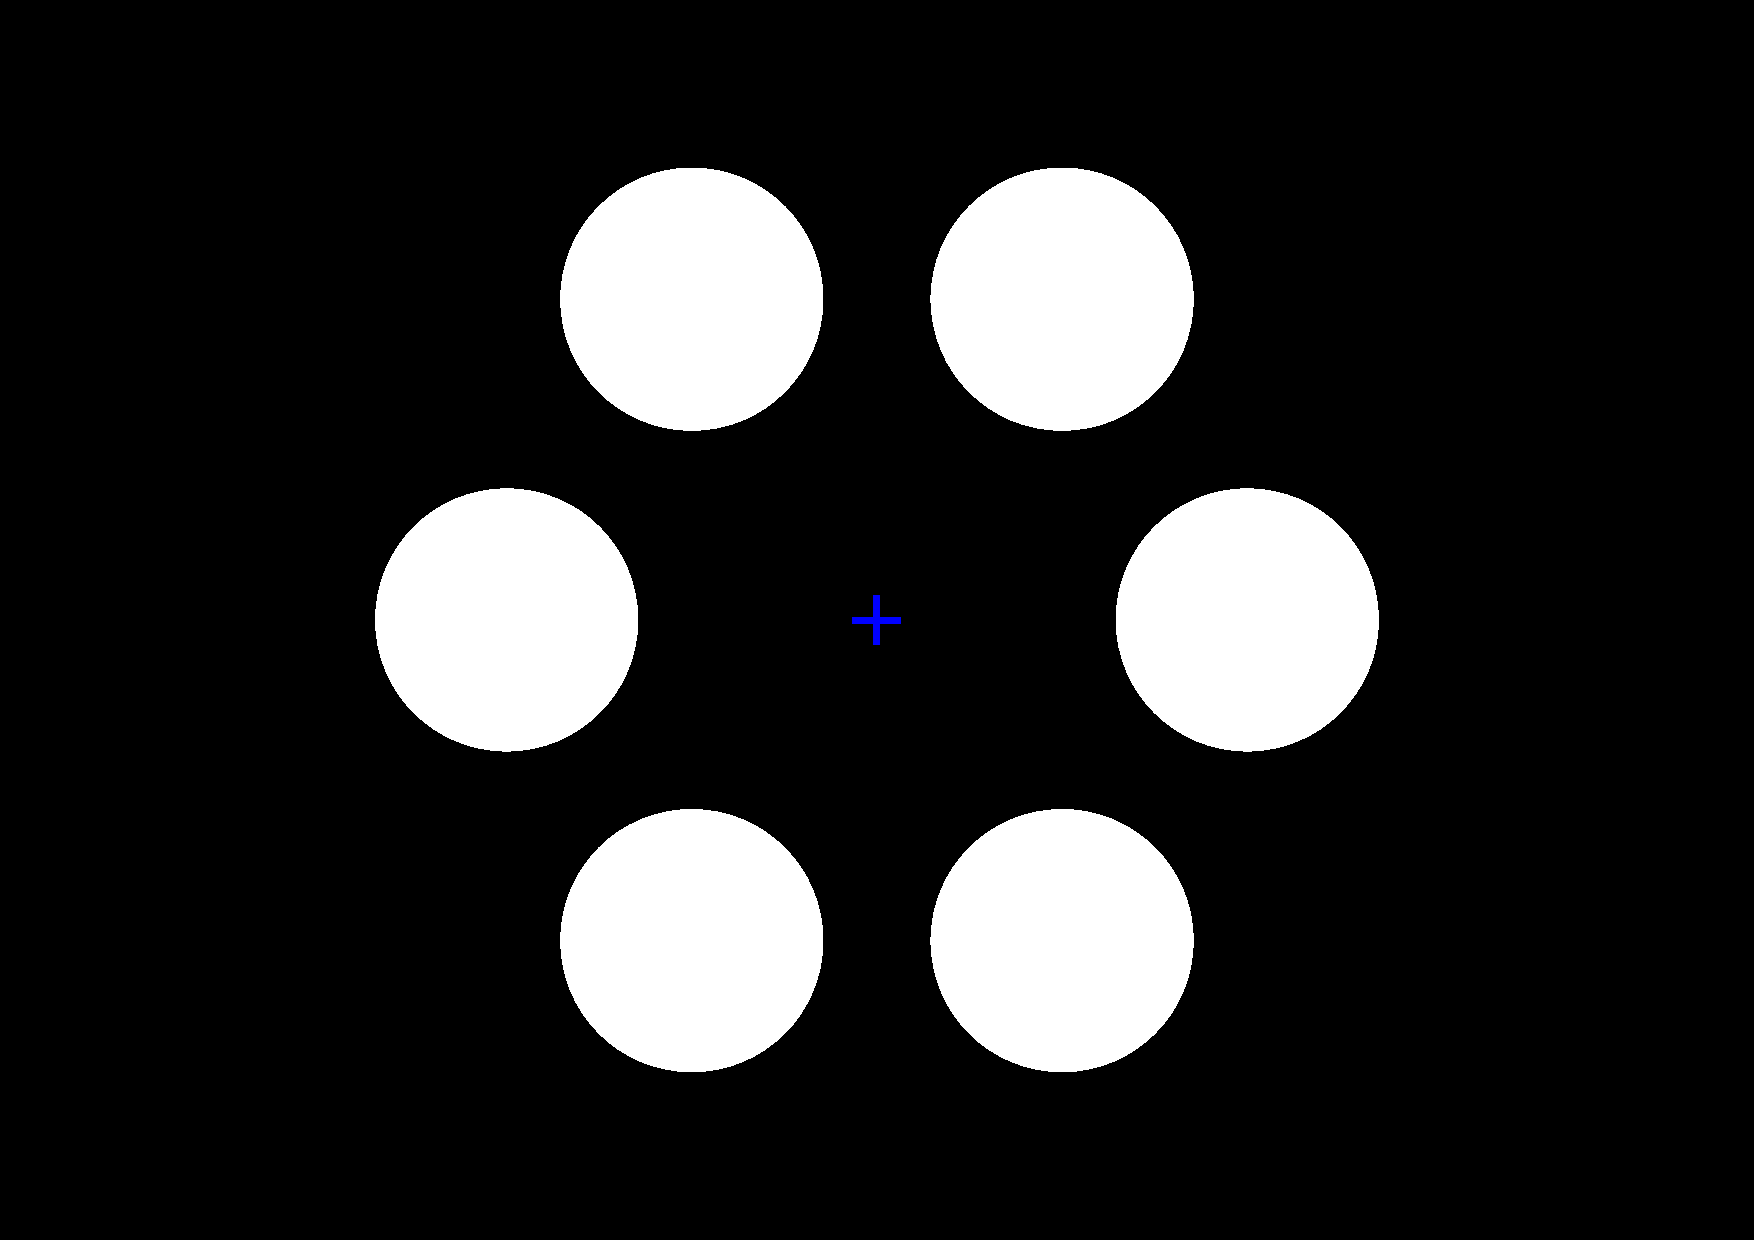
\includegraphics[width=\textwidth]{figures/stim_covert.pdf}
			\caption{In \emph{covert} \ac{vsa}, the fixation crosshair is placed in the
				center of the screen.}
		\end{subfigure}
		\smallskip

		\begin{subfigure}[b]{.45\linewidth}
			
\includegraphics[width=\textwidth]{figures/stim_free.pdf}
			\caption{In \emph{free} \ac{vsa}, no fixation crosshair is displayed.}
		\end{subfigure}\hfill%
		\begin{subfigure}[b]{.45\linewidth}
			
\includegraphics[width=\textwidth]{figures/stim_intense.pdf}
			\caption{Targets are intensified by enlarging them for 100 ms.}
		\end{subfigure}
	\end{minipage}

	\caption{Stimulation and recording setup for the oddball \ac{bci} experiment
		with different \ac{vsa} conditions}
	\label{fig:methods/stimulation/stimulation}
\end{figure*}
\todo{crosshair not visible, enlarge, white outline}

Three different \ac{vsa} settings were explored.
In the overt \ac{vsa} setting, the participant was instructed to fixate on the cued target or
to try this to the maximum extent of their visual skill, even if experiencing
slight discomfort.
In the covert \ac{vsa} setting, the participant was instructed to fixate on the center of the
screen, to the extent of their ability.
An additional \emph{free \ac{vsa}} setting was introduced.
Here, the participant was instructed to perform the task as they deemed most
comfortable.
This allowed us to investigate the user's natural way of operating the \ac{bci}
given their individual set of visual skills.
If the participant was not fully paralyzed, they were instructed not to move their head.
The cued \emph{split attention} setting proposed
by~\textcite{VanDenKerchove2024} was not studied here, as we were interested
in natural \ac{vsa} operation settings for gaze-impaired individuals.

To make the interface suitable for use by individuals with
participants with neurological conditions~\cite{FriedOken2020}, the amount of blocks was reduced to 6 per \ac{vsa} setting.
In order to decrease task difficulty, \ac{isi} was increased to 200 with added random jitter uniformly distributed
between -50 ms and 50 ms.
The experiment also started with a training block in each condition, where the
participant was instructed with oral feedback on their performance to ensure they
understood and were able to perform the task.


\subsection{\Ac{eeg} data collection \& preprocessing}

During the recording session, participants were positioned in their wheelchair in front of a table.
Stimuli were presented on an Acer Predator Helios laptop with an 18" screen (Acer,
Inc., Taiwan) placed at a 60 cm distance.
A Cedrus StimTracker (Cedrus Corp., CA, USA) ensured synchronization of stimuli with the
recorded \ac{eeg}.

\Ac{eeg} was recorded at 1000 Hz using the Neuroscan Neuvo portable amplifier (Compumedics Neuroscan,
Australia) connected to a second laptop for registration.
The \ac{eeg} headset used 18 active AgCl electrodes (EASYCAP GmbH, Germany) placed on a cap
according to the international 10-20 layout.
Using electrolyte gel, electrode impedances were reduced below 10 k$\Omega$.
Additionally, the \ac{eog} was recorded.

The \ac{eeg} was band-pass filtered between 0.5 and 16 Hz.
Bad channels were rejected using the RANSAC algorithm~\cite{Fischler1981}
and visual inspection.
Next, the \ac{eeg} was re-referenced to the average of mastoid electrodes TP9
and TP10, and \ac{ica} was performed to reject artifactual components based on
correlation with the \ac{eog} or by visual inspection.
Epochs were cut from -0.1 to 0.9 s relative to stimulus onset, and no baseline
correction was performed.

\subsection{\Acs{bci} decoding}

We evaluated the recorded \ac{eeg} data using the \ac{wcble}~\cite{VanDenKerchove2024}
and \ac{tlda}~\cite{Sosulski2022}
classifiers, as well as the Riemannian approach XDAWNCov+TS+LDA~\cite{Cecotti2017}.
For \ac{wcble}, a region of interest from 0 ms to 800 ms relative to stimulus
onset was used while the epoch was cropped to -100 ms to 900 ms. For the other
decoders, the epoch was cropped between 0 ms and 800 ms, which resulted in maximal
performance.
Decoding scores were obtained using 6-fold cross-validation where folds corresponded to
stimulation blocks.

\section{Results}



\subsection{Eye tracking analysis}
\label{sec:patients/outcomes/gaze}
Given their eye motor impairment as listed in~\cref{tab:patients/eye}, we aimed to clarify the
capabilities of the participants in performing overt \ac{vsa} and central gaze fixation and to
assess the relevance of these settings when gaze is not cued.
\Cref{fig:patients/gaze} maps gaze position relative to the targets
across conditions.
These results should be interpreted with care, as the eye tracker partially
relies on intact eye motility.
The participant's position relative to the eye tracker might have shifted
throughout the experimental session despite our best efforts, due to e.g.\ a
regular need for aspiration of the tracheostoma of some participants
\begin{figure*}[t]
	\resizebox{\linewidth}{!}{%
		\import{figures}{fig_gaze.pgf}%
	}%
	\caption{%
		Distribution of the recorded gaze position during the experimental session in the three \ac{vsa}
		conditions.
		Crosshairs represent stimulus positions, with positions cued during
		the given condition indicated in red.
		Subjects PB2 and PC4 preferred covert \ac{bci} operation, with PB2 resting gaze
		near the middle of the screen, and PC4 near the bottom.
	}%
	\label{fig:patients/gaze}
\end{figure*}
\todo{smoothing}
\todo{link to high resolution}

PA1 had relatively intact gaze control and was able to correctly perform the
cued overt and covert settings.
When gaze was uncued, he fixated on the cued target.
This was also mostly the case for PB1, although eye tracking revealed that he
chose not to perform central gaze fixation when cued in at least one of the
stimulation blocks. We were unable to record his gaze near the bottom-left
stimulus position, either due to eye tracker failure or because the participant
was not comfortable fixating on this position.
Eye tracker calibration did not succeed for subject PB4, but given the
transformation of gaze positions to the stimulus space, they were assumed to
be overtly performing the free task.

PB2 was able to perform overt \ac{vsa} and central fixation to some extent,
yet eye tracking shows a larger spread in gaze position compared to
PA1 and PB1.
In the free \ac{vsa} condition, however, she preferred to attend
stimuli covertly when the gaze was uncued.
This was confirmed by the participant.

The overt and central gaze fixation settings were also not properly adapted to
participant PC4.
In the free \ac{vsa} condition, eye tracker results show that his gaze was usually near the
bottom two targets, indicating some degree of covert or split \ac{vsa}.

Technical difficulties were encountered while recording gaze position with the
Tobii X2-30
Compact for participants PC2 and PC3, since they both had one eye that was
occluded respectively by the prism glass and the eyelid.
Both participants reported they could not fixate on some of the
stimuli.

\subsection{\Acs{bci} decoding performance}

\Cref{fig:patients/decode} shows cross-validated single-trial target selection
accuracy for the evaluated \ac{vsa} settings for the different decoders.
Accuracy results do not reveal a clear trend in classifier performance per
condition.
In the covert \ac{vsa} setting with cued central gaze fixation, performance
deteriorated overall.
Decoding performance for this task was at chance level ($\frac{1}{6}$) for
participants PB4, PC2 and PC3.
\todo{use target selection accuracy everywhere instead of performance}

\Ac{wcble} did not improve \ac{tlda} performance in the free \ac{vsa} setting, but
XDAWNCov+TS+LDA performance was slightly lower here (though not
significantly).
More interestingly, we noticed that performances of the decoders in free
\ac{vsa} were close to those in the overt \ac{vsa}.
A substantial decrease in performance from the overt setting to the free
setting was observed for subjects PC2, PC3 and PC4 who had the most severe eye
motor impairment.
For PB2, who relied on covert \ac{vsa} during the uncued free \ac{vsa}
according to gaze tracking setting, the decrease in performance was also
present.
\begin{figure*}[t]
	\sffamily
\begin{tikzpicture}[trim axis group left]

  \begin{groupplot}[
    group style={%
      group size=3 by 1,
      horizontal sep=10pt,
      ylabels at=edge left,
      yticklabels at=edge left,
    },
    ybar,
    ymin=0, ymax=105,
    ytick={0,20,40,60,80,100},
    xtick={0,1,2,3,4,5,6},
    xticklabels={PA1,PB1,PB2,PB4,PC2,PC3,PC4},
    xtick pos=bottom,
    ymajorgrids=true,
    xlabel={subject},
    ylabel={target selection accuracy (\%)},
    width=0.33\linewidth-5pt,
    scale only axis,
    /pgf/bar width=0.008\linewidth,
    cycle list/Set2-3,
    every axis plot/.append style={fill},
    every axis plot post/.append style={error bars/.cd, error bar style={color=gray}},
  ]

    \newcommand{\drawBarPlot}[2]{%
  	  \pgfplotstableread[col sep=comma]{data/decode_results_#1_#2_viz.csv}\datatable
  	  \addplot+[error bars/.cd, y dir=both, y explicit]
        table[
          x=subject_index,
          y=test_single_trial_accuracy-mean,
          y error minus=test_single_trial_accuracy-ci_minus,
          y error plus=test_single_trial_accuracy-ci_plus,
          col sep=comma
        ] {\datatable};
      }

    \newcommand{\drawRepMarker}[5]{%
  	  \pgfplotstableread[col sep=comma]{data/decode_results_#1_#2_viz.csv}\datatable
      \addplot+[only marks, mark=#5, mark size=2pt]
        table[
          x expr=\thisrow{subject_index} + #4,
          y=test_accuracy_reps_#3-mean,
          col sep=comma
        ] {\datatable};

    }

    \newcommand{\drawChanceLevel}{%
	    \draw[gray, dashed] (axis cs:-1,16.66666667) -- (axis cs:7,16.66666667);
    }

    \newcommand{\offset}{0.3}

    %% Plot overt
    \nextgroupplot[title=Overt \ac{vsa}]
    % Draw repetition performance
    \drawRepMarker{overt}{WCBLE}{5}{-\offset}{diamond}
    \drawRepMarker{overt}{tLDA}{5}{0}{diamond}
    \drawRepMarker{overt}{XDAWNCov+TS+LDA}{5}{\offset}{diamond}
    \drawRepMarker{overt}{WCBLE}{10}{-\offset}{square}
    \drawRepMarker{overt}{tLDA}{10}{0}{square}
    \drawRepMarker{overt}{XDAWNCov+TS+LDA}{10}{\offset}{square}
	  % Bar plot
    \drawBarPlot{overt}{WCBLE}
    \drawBarPlot{overt}{tLDA}
    \drawBarPlot{overt}{XDAWNCov+TS+LDA}
    % Draw chance level
    \drawChanceLevel

    %% Plot overt
    \nextgroupplot[title=Covert \ac{vsa}]
	  % Bar plot
    \addlegendimage{empty legend};
    \addlegendentry{\textbf{Decoder}};
    \drawBarPlot{covert}{WCBLE}
  	\addlegendentry{WCBLE};
    \drawBarPlot{covert}{tLDA}
  	\addlegendentry{tLDA};
    \drawBarPlot{covert}{XDAWNCov+TS+LDA}
  	\addlegendentry{XDAWNCov+TS+LDA};
    % Draw repetition performance
    \drawRepMarker{covert}{WCBLE}{5}{-\offset}{diamond}
    \drawRepMarker{covert}{tLDA}{5}{0}{diamond}
    \drawRepMarker{covert}{XDAWNCov+TS+LDA}{5}{\offset}{diamond}
    \drawRepMarker{covert}{WCBLE}{10}{-\offset}{square}
    \drawRepMarker{covert}{tLDA}{10}{0}{square}
    \drawRepMarker{covert}{XDAWNCov+TS+LDA}{10}{\offset}{square}
    %% Draw chance level
    \drawChanceLevel

    %% Plot overt
    \nextgroupplot[title=Free \ac{vsa}]
    % Draw repetition performance
    \drawRepMarker{free}{WCBLE}{5}{-\offset}{diamond}
    \drawRepMarker{free}{tLDA}{5}{0}{diamond}
    \drawRepMarker{free}{XDAWNCov+TS+LDA}{5}{\offset}{diamond}
    \drawRepMarker{free}{WCBLE}{10}{-\offset}{square}
    \drawRepMarker{free}{tLDA}{10}{0}{square}
    \drawRepMarker{free}{XDAWNCov+TS+LDA}{10}{\offset}{square}

	  % Bar plot
    \drawBarPlot{free}{WCBLE}
    \drawBarPlot{free}{tLDA}
    \drawBarPlot{free}{XDAWNCov+TS+LDA}
    %% Draw chance level
    \drawChanceLevel

  \end{groupplot}
\end{tikzpicture}%

	\caption{%
		Decoding performance in different \ac{vsa} settings reported as
		single-trial target selection accuracy (\%).
		Free \ac{vsa} is generally on par with performance in the overt \ac{vsa}
		setting.
		Performance in the covert \ac{vsa} setting with central gaze fixation is lower, but can
		be improved with the \ac{wcble} decoder.
		Whiskers indicate 95\% confidence intervals determined using 10,000 bootstrapping
		repetitions. Dashed line indicates the chance level accuracy. Diamond
		markers indicate target selection accuracy using the median score for five stimulation
		repetitions. Square markers indicate target selection accuracy for 10
		stimulation repetitions.
		($\frac{1}{6}$).
	}
	\label{fig:patients/decode}
\end{figure*}

\subsection{Cross-condition decoder training and evaluation}
\label{sec:patients/outcomes/cross}

As an alternative approach to selecting the most suitable decoder, we used
\ac{tlda} as the base decoder and verified whether performance could be improved
if \ac{bci} users with gaze impairment performed the decoder training session
session relying maximally on their residual gaze control.

\Cref{fig:patients/cross} shows that for participants PB1 and PC2 covert \ac{vsa} decoding
improved when training with overt \ac{vsa}.
Note that, according to eye tracking data, participant PB1, PB4, and PC4 did not
always perform cued central gaze fixation in the covert \ac{vsa} setting,
which might have affected the results.
\begin{figure*}[t]
	\sffamily
\begin{tikzpicture}[trim axis group left]

  \begin{groupplot}[
    group style={%
      group size=3 by 1,
      horizontal sep=10pt,
      ylabels at=edge left,
      yticklabels at=edge left,
    },
    ybar,
    ymin=0, ymax=100,
    ytick={0,20,40,60,80,100},
    xtick={0,1,2,3,4,5,6},
    xticklabels={PA1,PB1,PB2,PB4,PC2,PC3,PC4},
    xtick pos=bottom,
    ymajorgrids=true,
    xlabel={subject},
    ylabel={target selection accuracy (\%)},
    width=0.33\linewidth-5pt,
    scale only axis,
    /pgf/bar width=0.008\linewidth,
    cycle list/Set2-3,
    every axis plot/.append style={fill},
    every axis plot post/.append style={error bars/.cd, error bar style={color=gray}},
  ]

    \newcommand{\drawBarPlot}[2]{%
  	  \pgfplotstableread[col sep=comma]{data/cross_results_#1_#2_viz.csv}\datatable
  	  \addplot+[error bars/.cd, y dir=both, y explicit]
        table[
          x=subject_index,
          y=test_single_trial_accuracy-mean,
          y error minus=test_single_trial_accuracy-ci_minus,
          y error plus=test_single_trial_accuracy-ci_plus,
          col sep=comma
        ] {\datatable};
      }

    \newcommand{\drawChanceLevel}{%
	    \draw[gray, dashed] (axis cs:-1,16.66666667) -- (axis cs:7,16.66666667);
    }


    %% Plot overt
    \nextgroupplot[title=Overt \ac{vsa} evaluation]
	  % Bar plot
    \drawBarPlot{overt}{overt}
    \drawBarPlot{covert}{overt}
    \drawBarPlot{free}{overt}
    % Draw chance level
    \drawChanceLevel

    %% Plot overt

    \nextgroupplot[title=Covert \ac{vsa} evaluation]
	  % Bar plot
    \addlegendimage{empty legend};
    \addlegendentry{\textbf{Calibration setting}}

    \drawBarPlot{overt}{covert}
    \addlegendentry{overt \ac{vsa}};
    \drawBarPlot{covert}{covert}
    \addlegendentry{covert \ac{vsa}};
    \drawBarPlot{free}{covert}
    \addlegendentry{free \ac{vsa}};
    %% Draw chance level
    \drawChanceLevel

    %% Plot overt
    \nextgroupplot[title=Free \ac{vsa} evaluation]
    % Draw repetition performance
	  % Bar plot
    \drawBarPlot{overt}{free}
    \drawBarPlot{covert}{free}
    \drawBarPlot{free}{free}
    %% Draw chance level
    \drawChanceLevel

  \end{groupplot}
\end{tikzpicture}%

	\caption{
		Decoding performance when calibrating the \ac{tlda} decoder in a given \ac{vsa}
		setting, and evaluating it in another, reported as
		single-trial \ac{rocauc}.
		Whiskers indicate 95\% confidence intervals determined using 10,000 bootstrapping
		repetitions.
		For participants PA1, PB2, and PC3, performance in the covert \ac{vsa} setting with central gaze fixation
		improved when calibrating with overt gaze fixation.
	}
	\label{fig:patients/cross}
\end{figure*}

\section{Discussion}

This study investigated the feasibility of a gaze-independent visual oddball
\acp{bci} for individuals with \ac{sspgi}.
While covert \ac{vsa} with cued, central gaze fixation resulted in reduced BCI
performance, likely due to increased task load, accuracy in free \ac{vsa} where gaze position is uncued can
yield performance comparable to explicitly cued overt \ac{vsa} for some
participants.
This suggests that the evaluated participants naturally integrate residual gaze control.
Training with cued, overt \ac{vsa} can improve subsequent performance in covert
or free \ac{vsa} conditions,
highlighting the potential benefits of leveraging this residual eye motor control
during the decoder training phase.
While gaze-independent BCIs show promise for individuals with \ac{sspgi},
usability and comfort remain critical considerations for real-world applications.
These results provide important insights into the optimization of visual BCIs for individuals with severe motor impairments and underscore the need for further research into adaptive decoding strategies and user-centered design.
\todo{move to conclusion/check if it is present in conclusion and last part of the discussion}

\subsection{Gaze-independent operation \& decoding}
Due to the heterogeneous nature of the participants' conditions and the limited
number of participants, it is difficult to draw general conclusions.
This study should therefore be seen as a collection of case studies,
highlighting different obstacles encountered in developing gaze-independent
visual oddball \acp{bci} for individuals with \ac{sspgi}.
Nevertheless, we highlight some aspects that might be
of interest for the further development of this class of \acp{bci}.

True \emph{gaze-independent} visual \acp{bci} should not rely on gaze fixation.
Hence, our analysis centers around the free \ac{vsa} condition.
Eye tracking results presented in \cref{sec:patients/outcomes/gaze}
confirm our assumption that voluntary covert \ac{vsa} can
occur in individuals with \ac{sspgi}.
We also confirmed part of the results presented by \textcite{VanDenKerchove2024},
which state that decoding of covert \ac{vsa} with central gaze
fixation can be improved by accounting for latency jitter. We showed that this
also holds for some individuals with \ac{sspgi}, with PA1 and PC4 as examples.

Contrary to our assumptions, we have shown that accounting for latency jitter does not
necessarily improve covert \ac{vsa} when gaze fixation is not cued.
One possible explanation is that actively performing central gaze fixation
increases task load.
This, in turn, can reduce overall performance, even though the participant might
have otherwise performed covert \ac{vsa}, but would not be occupied with
maintaining strict central gaze fixation.
This extra task demand is not present in the free \ac{vsa} condition, so
there is less performance to be gained.
Furthermore, cued central gaze fixation combined with counting flashing stimuli
in the visual periphery is an explicit example of a dual task.
Dual tasks have been shown to increase P3 latency
jitter~\cite{Polich2007,Arico2014, VanDenKerchove2024},
which is what \ac{wcble} accounts for.
Hence, increased P3 jitter might be more related to maintaining central gaze fixation
than to the actual covert \ac{vsa} aspect.

The seemingly stable performance across overt and free \ac{vsa} could be
misinterpreted as an indication that the Hex-o-Spell \ac{bci} already works
well for individuals with \ac{sspgi}, and no optimization is
needed.
However, we assume that overt \ac{vsa} performance was also decreased in some
subjects or for some blocks if the participant was not able to comfortably
perform the task.
Nevertheless, the large difference between the free \ac{vsa} setting and the
covert \ac{vsa} setting
with central gaze fixation is food for thought about the applicability of
solutions developed with central fixation in mind.

Individuals with all except the most severe gaze impairments will likely retain
some capability to direct their gaze in visual \ac{bci} operation, which can
drastically boost performance.
Subject PB2 exemplifies this: his free \ac{vsa} performance is above the covert
\ac{vsa} performance, and eye tracking showed that he relied mostly
on overt \ac{vsa} when cued to do so, and mostly on covert \ac{vsa} when
gaze was uncued.
This is also supported by our results on cross-condition decoder training and evaluation presented
in \cref{sec:patients/outcomes/cross}, which show that leveraging residual
eye motor control to fixate targets during the decoder training phase can improve
performance in some settings.
This is likely due to the increased P3 component amplitude in overt \ac{vsa},
which improves the discriminative power of a classifier trained on this data.
Cueing this overt gaze fixation only during the decoder training phase leaves the user
free to operate in the manner that is most comfortable in the
operation phase.
Early VEPs in the training data could also contribute in those cases where the participant was not
able to perform covert \ac{vsa} with central gaze fixation.

\subsection{Clinical implications}
The population of individuals with \ac{sspgi} is sparse, yet is regularly
confronted with major challenges.
As opposed to individuals in a vegetative or severe minimally conscious state,
they demonstrably have the intent and capability to communicate their thoughts
and desires to their clinicians, caregivers and social network.
These capabilities, however, are severely limited by their condition,
reducing the effectiveness and efficiency of communication.
Hence, finding a way to fill in this gap is a major issue in the care of
individuals with \ac{sspgi}.

Our work shows that some patients might benefit from visual \acp{bci}
for home use or in the clinical setting.
While the proposed communication protocol is a proof of concept with a limited degree
of freedom, it is a step towards applications like textual communication and
environment or home automation control that inherits the relatively high
information transfer rate of visual \acp{bci}.

Furthermore, our experiments revealed that the required technology and its
potential applications were generally well received by the participants and their
environment.
While the necessary visual attention task can be taxing if performed for
extended
periods of time, participants indicated that this was outweighed by the
potential to communicate in a more automated and autonomous way compared to
their current \ac{aac} solutions, which often required the help of a trained caregiver.

\subsection{Limitations}

Despite the insights gained on gaze-independent \ac{bci} approaches, certain limitations must be addressed in future research.
First and foremost, this study works with a limited sample size, which
does not represent the full spectrum of individuals with
\ac{sspgi} and their specific symptoms and skills.
Individuals with \ac{fa} met the inclusion criteria, but they are usually not
considered one of the typical interest groups for \ac{bci} communication assistive
technology, partly due to the rarity of the disease and partly due to its
progression.
It would be most interesting to verify these results with individuals with
\ac{lis} and no eye movement capability at all.

Another limiting factor is the difficulty experienced in correctly interpreting eye
tracker results in studies with individuals with gaze impairments.
If eye tracking is possible at all, it is not guaranteed that the user is able
to successfully perform the calibration procedure.
Further experiments should be carried out with a stationary eye tracker with
more advanced capabilities, although systems using a head fixator or headrest
should be avoided.
This is not practical when working with
wheelchair-bound individuals who might have undergone a tracheostomy and may
suffer from spasticity.
\todo{Maybe to better relate performance to the extent and nature of the impairment}

In this study, user comfort in the different conditions was not objectively
measured.
Instead, it was assumed that participants operated most comfortably in the free
\ac{vsa} condition.
Even though participants reported that they could comfortably operate the
system, this must be confirmed with more quantitative assessments.
To properly contextualize performance results, they should be coupled with
metrics evaluating the full scope of the user's requirements, with measures of
usability, comfort and perceived effort, like the NASA Task Load
Index~\cite{Hart2006} and other metrics proposed in the user-centered design
framework for \acp{bci}~\cite{Kuebler2014}.
Performance might, after all, be traded off for user comfort.
The perception of this type of \ac{bci} by the user might also be influenced by
performing the experiment in an on-line manner, providing immediate feedback
after selection and thus closing the loop.
%Eye motor disability could also have been assessed more
%objectively~\cite{FriedOken2020}, using, e.g.,
%the Revised Coma Recovery Scale~\cite{Giacino2004} or the NSUCO
%oculomotor exam~\cite{Maples1992}.

Finally, the stimulation procedure parameters
from~\textcite{VanDenKerchove2024} were adapted to make the counting task
accessible to the \ac{bci} users with \ac{sspgi}.
However, the number of repetitions and the \ac{isi} were not optimized to achieve
maximal \ac{itr}.
An interface that aims to maximize \ac{itr} could necessitate more or faster
gaze redirections, which might result in different conclusions regarding the
comfort and the impact of the retained visual skills.

\acresetall
\section{Conclusion}
This study explored the usability of \ac{eeg}-based gaze-independent visual BCIs in
individuals with \ac{sspgi}, focusing on the impact of eye motor impairments
on performance.
Our results demonstrate that a visual \ac{bci} gaze-independent operation is feasible
for some of these individuals.
They might either achieve sufficient decoding accuracy despite their eye
motor impairment, or performance can be enhanced by careful, individual
adaptation the decoding strategies.
The free \ac{vsa} condition yielded performance comparable to overt \ac{vsa} in some participants, suggesting that users may naturally integrate residual gaze control.
Additionally, training under overt \ac{vsa} conditions improved performance in
subsequent covert or free \ac{vsa} operation, highlighting the potential benefits of
leveraging residual eye motor capabilities during decoder training.
While these findings are promising, future work should include larger
participant groups, refine stimulation paradigms, and incorporate
user-centered assessments of comfort and usability.
Ultimately, optimizing gaze-independent BCI designs could enhance communication
options for individuals with severe motor and speech impairments, particularly
those who struggle with conventional eye-tracking technologies.


\section*{Acknowledgements}
AVDK is funded by the special research fund of the KU Leuven (GPUDL/20/031).
MMVH is supported by research grants received from the European Union’s
Horizon Europe Marie Sklodowska-Curie Action program
(grant agreement No. 101118964), the European Union’s Horizon 2020 research and
innovation program (grant agreement No. 857375), the special research fund of
the KU Leuven (C24/18/098), the Belgian Fund for Scientific Research – Flanders
(G0A4118N, G0A4321N, G0C1522N), and the Hercules Foundation (AKUL 043).

The authors acknowledge the support by the RITMEA project co-financed by the
European Union with the European Regional Development Fund, the French state,
and the Hauts-de-France Region Council.
\printbibliography

\end{document}
